\documentclass[12pt,a4paper]{article}
\usepackage[a4paper,left=2cm,right=2cm,top=3cm,bottom=3cm]{geometry}
\usepackage[utf8]{inputenc}
\usepackage[T1]{fontenc}
\usepackage{amsmath}
\usepackage{nicefrac}
\usepackage{amssymb}
\usepackage{float}
\usepackage{graphicx}
\usepackage[german]{babel}
\title{Untersuchung Uplifter: Ausfall der Messkette X-201---X-135}

\begin{document}
	\maketitle
	\newpage
	\section{Ausgangslage}
	Bei der Firma Uplifter wird eine Messkette bestehend aus dem Sensor X-135 und dem Verstärker X-201-IN09 zur Überwachung der Achslast zum Schutz vor Kippen in den Scheibenhebe-Roboter eingesetzt. Die analoge Messkette liefert ein Signal in Milliampere mit einem \textit{Living Zero} von 4mA. Nach dem Verbau der Messkette nimmt Uplifter eine Kalibration mit Totgewichten vor. \\
	Während der Fertigung und den damit verbundenen Tests oder teils auch später im Feld fallen teilweise Messketten aus. Die Verstärker liefern dann ein Signal $< 4mA$, wodurch der Sensor für die Steuerung dann als \textit{Offline} gilt.\\
	Ein von Uplifter angemerkter Verdacht besteht darin, dass die Messkette teilweise ausfällt, nachdem die Maschine mit dem Gabelstapler ausgeladen wurde. Der Verdacht liegt darin, dass beim Aufsetzten der Maschine auf dem Boden kurzzeitig hohe Kräfte / Spitzen auf den Sensor und somit auf die Messkette wirken.
	Die Firma Uplifter hat beim vor-Ort-Besuch vom 05.10.2023 zwei defekte Messketten für die Analyse retourniert.
	\section{Untersuchungen}
	In einem ersten Schritt wurden die zwei defekten Messketten analysiert. Anschliessend wurde ein Testaufbau aufgesetzt, um die Messketten in der Uplifter-Konfiguration im Dauerbetrieb zu testen.
	\subsection{Analyse der defekten Messketten}
	Die Analyse der beiden retournierten Messketten hat ergeben, dass in beiden Fällen eine Schutzdiode, welche unmittelbar im Speisungspfad liegt und die Speisung/Steuerung vor Rückströmen schützt, defekt ist. 
	\subsection{Testaufbau}
	Uplifter hat die Ausfallquote der Messkette auf ca. 50\% geschätzt. Um eine hinreichend große Stichprobe für den Versuchsaufbau zu haben, wurde eine Wahrscheinlichkeit, dass \textit{mindestens ein} Verstärker ausfällt, mit 95\% angenommen. Daraus ergibt sich:
	\begin{equation}
		1 - 0.5^n \ge 0.95 \leftrightarrow 0.5^n  \le 0.05 \rightarrow n \ge log_{0.5}(0.05) = 4.32
	\end{equation} 
	Mit einer Losgrösse von 5 und der Prämisse, dass 50\% der Messketten in den Anfangsstunden in Betrieb ausfallen, liegt also die Wahrscheinlichkeit, dass mindestens 1 Verstärker ausfällt, bei 
	\begin{equation}
		1-0.5^5 = 0.96875 \approx 96.9\%
	\end{equation}
	Für den Testaufbau wurden 5 Messketten mit dem Stand der letzten Uplifter-Auslieferungen sowie 5 Messketten mit einer Printmodifikation auf einer geerdeten Platte aufgebaut und mit einem Labornetzteil mit 24V betrieben. Anstelle der Sensoren wurden DMS-Simulatoren an die Verstärker angeschlossen, damit grosse Signalsprünge ohne phyischen Aufwand generiert werden können.\\
	Um den Stand der Signalausgänge der Verstärker zu visualisieren, wurde eine THT-LED in den Stromausgangspfad verbaut. Die Leuchthelligkeit ist hierbei proportional zum Ausgangsstrom, welcher je nach anliegendem Sensorsignal im Bereich von 4...20mA liegt.\\
	\begin{figure}[H]
		\centering
		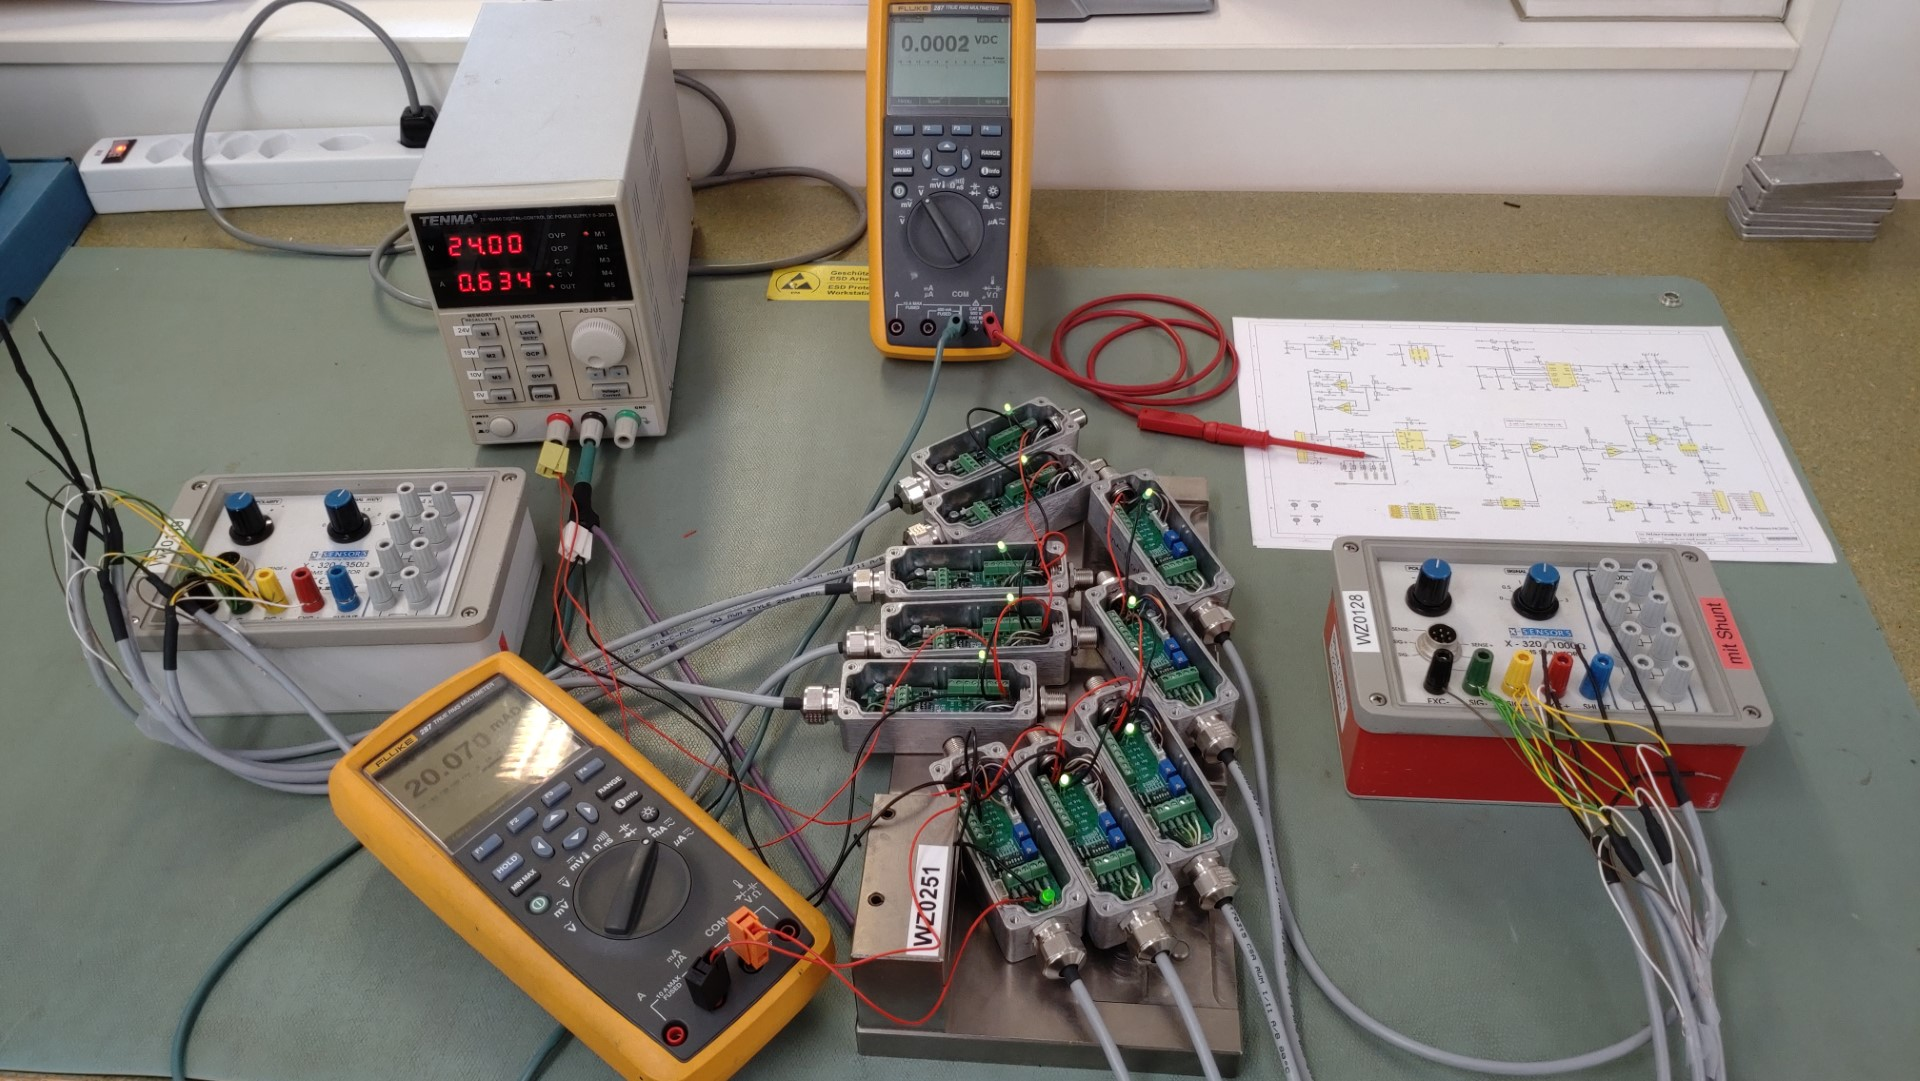
\includegraphics[width=1\linewidth]{imgs/Uplifter_Aufbau_1}
		\caption{Testaufbau für Dauerbetrieb}
		\label{fig:uplifteraufbau1}
	\end{figure}\noindent
	\subsection{Resultate}
	Im Dauertest wurde das Sensorsignal von Zeit zu Zeit über die Simulatoren sprunghaft im Bereich von 0...4 $\nicefrac{mV}{V}$ verstellt. Die X-135 Sensoren, welche aktuell bei Uplifter eingesetzt werden, liefern Signale im Bereich von 0...1.5. $\nicefrac{mV}{V}$ und würden sich bei einer Last, welche 4 $\nicefrac{mV}{V}$ erzeugt, plastisch verformen. Mit den Simulatoren können somit massive Überlasten simuliert werden. Weiter wurden die Verstärker bei unterschiedlichen anliegenden Sensorsignalen tariert.\\
	Über einen Zeitraum von 72h konnte jedoch kein Ausfall ``provoziert'' werden, womit die Einbausituation bei Uplifter sowie die elektrischen Eigenschaften der steuerungsseitig an die Messkette angeschlossenen Elemente genauer überprüft werden sollten.
	
\end{document}